\subsection{Project Requirements} \label{label:projectRequirements}
Number of functional and non-functional requirements have been identified and prioritized using MoSCoW approach during the design stage. 

\subsubsection{MoSCoW method}
As shown in the following sections, large number of requirements have been identified for ALIAS. However, due to the time limitation of the project, not all of them will delivered. The final software deliverable will be a minimum viable product: a product with enough features that can be delivered in the specified time line. Furthermore, the selected features should be critical to the system, introducing important functionality into the application \citep{mvp}.

Thus, in order to select the minimum viable product for this project, all the requirements have been prioritized using MoSCoW approach. The approach originated from DSDM methodology (Dynamic Software Development Method) and uses four levels to define the priority \citep{moscow}:

\begin{enumerate}
	\item \textbf{M}ust Have - features that must be included in the application by the end of the project. It defines the minimum usable subset of functionalities 
	\item \textbf{S}hould Have - defines non-critical functionality that is not necessarily required in the final product, but is of high value
	\item \textbf{C}ould Have - any features that could improve the final product and could potentially be included in the scope of the project without incurring too much effort or cost.
	\item \textbf{W}on't Have - any features that have been identified in the requirements analysis, but will be excluded from the scope of this project. Those features can be revisited and added in future work.
\end{enumerate}

Hence, any features categorized as \textit{Must Haves} are critical to the project and they have to be implemented during this project. Failing to do so might result in the project to be considered as failed. 

\subsubsection{Functional Requirements}

\paragraph{Solver} \mbox{} \\

Most of functional requirements have been created based on solver requirements for International Competition on Computational Models of Argumentation 2017. Furthermore, those requirements can be characterized based on their functionality:
\begin{itemize}
	\item Computational functionality - those include all different types of semantics and individual tasks related to them. For example, a requirement will exist for the solver to compute the stable extensions of the given argumentation framework. However, this could be further split up into separate tasks: compute all extensions, some extensions, evaluate if the given argument is skeptically or credulously accepted.
	\item Solver functionality - those include additional requirements that the solver should have. They might include requirements like solver should be able to read \textit{tgf} file and parse the argumentation framework from them, etc.
\end{itemize}

In terms of the computational functionality, ALIAS is required to solve all semantics identified in section \ref{sec:argumentationSemantics}, which are as follow: complete, stable, preferred and grounded extensions \citep{dung1995}, stage \citep{verheij1996two}, ideal \citep{dung2007computing}, and semi-stable \citep{caminada2006semi} semantics. Although seven individual semantics have been identified as the requirements for the solver, only three of them: complete, stable and preferred, have been classified as \textit{Mush Have} in terms of MoSCoW approach. The proposed semantics are part of the original group of extensions introduced by \citet{dung1995} in his paper. 

Furthermore, as mentioned above, there are number of tasks that the solver should be able to perform for each semantic and as seen in the section \ref{approaches}, those are as follow:
\begin{enumerate}
	\item Given an abstract argumentation framework compute some of the extensions
	\item Given an abstract argumentation framework compute all extensions
	\item Given an abstract argumentation framework and some argument, decide whether the given argument is credulously accepted
	\item Given an abstract argumentation framework and some argument, decide whether the given argument is skeptically accepted
\end{enumerate}

Above tasks are relevant to all semantics with exception to grounded and ideal extensions, where only tasks 1 and 3 can be performed. Hence, it brings up the overall number of tasks for all semantics to 24 separate tasks. Thus, to deliver solution with the most value, for the extensions categorized as \textit{Must Have}, only tasks to compute all extensions have been categorized as \textit{Must Haves}. The remaining tasks for each of them have been classified as \textit{Should Have}. Furthermore, computing all Semi-Stable and Stage extensions have been categorized as \textit{Could Have}, with all the remaining tasks and extensions as \textit{Won't Have}. This can be seen in table \ref{table:moscowSemanticRequirements} and further in the appendix \ref{appendix:requirementAnalysis}. 


% Please add the following required packages to your document preamble:
% \usepackage{multirow}
\begin{table}[]
	\centering
	\caption{MoSCoW qualifications of semantic based requirements}
	\label{table:moscowSemanticRequirements}
	\begin{tabular}{|l|l|l|}
		\hline
		\textbf{Semantic}            & \textbf{Task}                                   & \textbf{MoSCoW} \\ \hline \hline
		\multirow{4}{*}{Complete}    & Compute all extensions                           & Must Have       \\ \cline{2-3} 
		& Compute some extensions                          & Should Have     \\ \cline{2-3} 
		& Decide if argument is credulously accepted & Should Have     \\ \cline{2-3} 
		& Decide if argument is skeptically accepted & Should Have     \\ \hline
		\multirow{4}{*}{Preferred}   & Compute all extensions                           & Must Have       \\ \cline{2-3} 
		& Compute some extensions                          & Should Have     \\ \cline{2-3} 
		& Decide if argument is credulously accepted & Should Have     \\ \cline{2-3} 
		& Decide if argument is skeptically accepted & Should Have     \\ \hline
		\multirow{4}{*}{Stable}      & Compute all extensions                           & Must Have       \\ \cline{2-3} 
		& Compute some extensions                          & Should Have     \\ \cline{2-3} 
		& Decide if argument is credulously accepted & Should Have     \\ \cline{2-3} 
		& Decide if argument is skeptically accepted & Should Have     \\ \hline
		\multirow{4}{*}{Semi-Stable} & Compute all extensions                           & Could Have      \\ \cline{2-3} 
		& Compute some extensions                          & Won't Have      \\ \cline{2-3} 
		& Decide if argument is credulously accepted & Won't Have      \\ \cline{2-3} 
		& Decide if argument is skeptically accepted & Won't Have      \\ \hline
		\multirow{4}{*}{Stage}       & Compute all extensions                           & Could Have      \\ \cline{2-3} 
		& Compute some extensions                          & Won't Have      \\ \cline{2-3} 
		& Decide if argument is credulously accepted & Won't Have      \\ \cline{2-3} 
		& Decide if argument is skeptically accepted & Won't Have      \\ \hline
		\multirow{2}{*}{Grounded}    & Compute all extensions                           & Won't Have      \\ \cline{2-3} 
		& Decide if argument is credulously accepted & Won't Have      \\ \hline
		\multirow{2}{*}{Ideal}       & Compute all extensions                           & Won't Have      \\ \cline{2-3} 
		& Decide if argument is credulously accepted & Won't Have      \\ \hline
	\end{tabular}
\end{table}


The above classification is only concerned with the argumentation semantics and its tasks. Other requirements have been identified that although are not concerned with solving the abstract argumentation semantics are needed for the solver and can improve the system. As an example, ALIAS should be able to read parse the argumentation framework from the provided file, like \textit{tgf} or \textit{apx}, or from dot graph or even the database. Furthermore, the user should be able to save created argumentation framework in different formats for future use. 

Although original implementation of ALIAS provides a certain aspects of those requirements, during the development of the new version, the architecture of the system and its implementation will have to be reviewed and modified to allow for the changes to the main solver. Thus, the functional requirements concerned with the solver can be seen in table \ref{table:functReqFunctionality}.

% Please add the following required packages to your document preamble:
% \usepackage{graphicx}
\begin{table}[]
	\centering
	\resizebox{\textwidth}{!}{%
		\begin{tabular}{|p{0.5cm}|p{10cm}|p{2.5cm}|}
			\hline
			\textbf{Id} & \textbf{Requirement} & \textbf{MoSCoW}  \\ \hline \hline
			1 & Should read and parse AF from provided tgf file & Must have \\ \hline
			2 & Should read and parse AF from provided apx file & Should have \\ \hline
			3 & Should read and parse AF from provided JSON file & Could Have \\ \hline
			4 & Should read and parse AF from provided D3.js file & Could Have \\ \hline
			5 & Should read and parse AF from provided dot file & Could Have \\ \hline
			6 & Should read and parse AF from provided networkx object & Could Have \\ \hline
			7 & Should read and parse AF from provided SQL database & Could Have \\ \hline
			8 & User should be able to create a new empty AF & Must have \\ \hline
			9 & User should be able to add argument to AF & Must have \\ \hline
			10 & User should be able to add list of arguments to AF & Could Have \\ \hline
			11 & User should be able to add attack to AF & Must have \\ \hline
			12 & User should be able to add list of attacks to AF & Could Have \\ \hline
			13 & User should be able to draw AF as networkx graph & Should have \\ \hline
			14 & User should be able to export the AF in JSON format & Must have \\ \hline
		\end{tabular}%
	}
	\caption{Functional Requirements for Solver functionality}
	\label{table:functReqFunctionality}
\end{table}

\paragraph{Web User Interface} \mbox{} \\
Apart from the requirements for the solver itself, there are number of requirements for the Web UI. The User Interface does not introduce any new functionality in terms of the solver abilities, however it provides a facade that can be used to work on, and modify argumentation frameworks in ALIAS and request certain extensions to be computed. 

% Please add the following required packages to your document preamble:
% \usepackage{longtable}
% Note: It may be necessary to compile the document several times to get a multi-page table to line up properly
\begin{longtable}[c]{|p{0.5cm}|p{10cm}|p{2.5cm}|}
	\hline
	\textbf{Id} & \textbf{Requirement} & \textbf{MoSCoW} \\ \hline \hline
	\endfirsthead
	%
	\endhead
	%
	1 & User should be able to load predefined example AFs & Must have \\ \hline
	2 & User should be able to create a new AF from UI & Must have \\ \hline
	3 & User should be able to add argument from UI & Must have \\ \hline
	4 & User should be able to add attack from UI & Must have \\ \hline
	5 & User should be able to upload AF in tgf format & Should Have \\ \hline
	6 & User should be able to upload AF in apx format & Could Have \\ \hline
	7 & User should be able to uplaod AF in JSON format & Won't Have \\ \hline
	8 & User should be able to export AF in tgf format & Won't Have \\ \hline
	9 & User should be able to export AF in apx format & Won't Have \\ \hline
	10 & User should be able to export AF in JSON format & Won't Have \\ \hline
	11 & User should be able to request all Complete Extensions of AF & Must have \\ \hline
	12 & User should be able to check if given argument is credulously accepted in complete extensions & Could Have \\ \hline
	13 & User should be able to check if given argument is skeptically accepted in complete extensions & Could Have \\ \hline
	14 & User should be able to request all Stable Extensions of AF & Must have \\ \hline
	15 & User should be able to check if given argument is credulously accepted in Stable extensions & Could Have \\ \hline
	16 & User should be able to check if given argument is skeptically accepted in Stable extensions & Could Have \\ \hline
	17 & User should be able to request all Preferred Extensions of AF & Must have \\ \hline
	18 & User should be able to check if given argument is credulously accepted in Preferred extensions & Could Have \\ \hline
	19 & User should be able to check if given argument is skeptically accepted in Preferred extensions & Could Have \\ \hline
	20 & User should be able to request all Semi-Stable Extensions of AF & Won't Have \\ \hline
	21 & User should be able to check if given argument is credulously accepted in Semi-Stable extensions & Won't Have \\ \hline
	22 & User should be able to check if given argument is skeptically accepted in Semi-Stable extensions & Won't Have \\ \hline
	23 & User should be able to request all Stage Extensions of AF & Won't Have \\ \hline
	24 & User should be able to check if given argument is credulously accepted in Stage extensions & Won't Have \\ \hline
	25 & User should be able to check if given argument is skeptically accepted in Stage extensions & Won't Have \\ \hline
	26 & User should be able to request all Grounded Extensions of AF & Won't Have \\ \hline
	27 & User should be able to check if given argument is credulously accepted in Grounded extensions & Won't Have \\ \hline
	28 & User should be able to request all Ideal Extensions of AF & Won't Have \\ \hline
	29 & User should be able to check if given argument is credulously accepted in Ideal extensions & Won't Have \\ \hline
	\caption{Web UI Functional Requirements}
	\label{table:webUiRequirements}\\
\end{longtable}

As can be seen in table \ref{table:webUiRequirements}, the requirements for the Web User Interface extend requirements for the main solver. However, since the Web UI will be build on top of ALIAS, it is critical to treat it separately in terms of requirements. 

\subsubsection{Non-Functional Requirements}
Apart from all functional requirements, number of non-functional requirements have also been identified. Those are mostly concerned with the performance and scalability of the proposed solution. Although those do not bring any tangible value to the finished system, those requirements are critical to produce the high performance and scalable system that could match existing solvers in terms of computation time. Hence, the non-functional requirements can be classified as follow:

\begin{enumerate}
	\item Performance - the overall performance of the application when performing certain tasks, especially computing extensions of given Argumentation Framework
	\item Scalability - ability to scale appropriately for larger Argumentation Frameworks
	\item Ease of Use - the ease of setup and use of the application 
	\item Desing - concerned with the design of the Web User Interface
\end{enumerate}

Performance, scalability and ease of use requirements are applied not only to the ALIAS application, but also to the Web User Interface. 

\paragraph{Performance and Scalability} \mbox{} \\

In terms of performance and scalability, the requirement for the ALIAS is to be able to cope with argumentation frameworks of any size. User should be confident that the application will be able to provide the correct results all time, no matter the size of provided framework. Although, it is difficult to convert it into tangible requirements, the attempt has been made to specify brackets for different sizes of argumentation frameworks: 

\begin{enumerate}
	\item Small - up to 20 arguments and relations
	\item Medium - from 20 up to 100 arguments and relations
	\item Large - above 100 arguments 
\end{enumerate}

However, the above classification is only concerned with the size of graph generated from the argumentation framework. Although this can usually correspond to the complexity of the framework, it is not always the case. For example, argumentation framework shown in figure \ref{fig:mediumAF} consist of only 41 arguments and 73 attacks. However, the testing of proposed solutions showed that although the argumentation framework is of medium size, the complexity of relations between the arguments proved to be challenging due to many arguments defending themselves. Thus, the above classification will only be used for establishing basic requirements for the application to be able to handle all types of argumentation frameworks. 

\begin{figure}[h]
	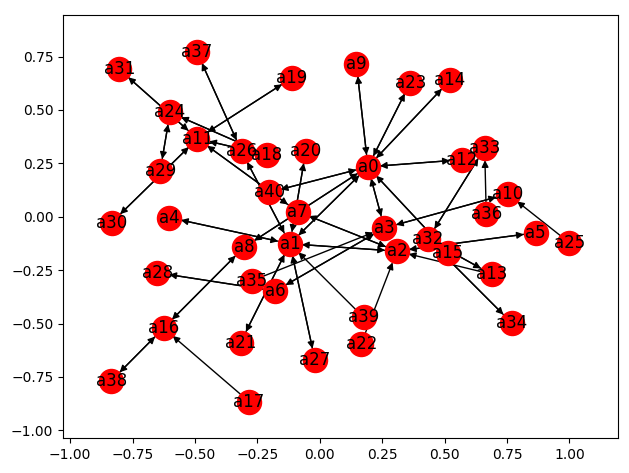
\includegraphics[width=\textwidth]{medium}
	\caption{Medium sized argumentation framework}
	\label{fig:mediumAF}
\end{figure}

In terms of ALIAS Web Extension, the performance and scalability requirements are mostly concerned with the time required to load and render any given Argumentation Framework. User should be able to display and work on large graphs in the UI. On the other hand, the performance of any operation on the given Argumentation Framework will be highly dependent on the performance of ALIAS.

\paragraph{Ease of Use} \mbox{}\\

Another aspect of non-functional requirements is the ease of use of the application. Original ALIAS application has been implemented in Python, an interpreted, high-level programming language \citep{millman2011python}. Although Python has been designed as the general purpose language, it became very popular. And with the libraries like NumPy and SciPy, it became a popular choice for high-level scientific code development \citep{perez2011python}. Thus, the Python implementation of abstract argumentation semantics solver without the need to setup the environment in any way prior to using it would be beneficial. Being able to install the ALIAS from the PyPi, the Python package manager \citep{pypi}, and use it 'out of the box', gives it an advantage over other solvers.

Ease of use requirement is further addressed by the ALIAS Web Interface. By providing the User Interface, the application is more readily available for anyone wishing to explore and work with Argumentation Frameworks. Web UI removes any need for programming skills as the user would be able to interact with ALIAS through the API.

\paragraph{Design} \mbox{} \\
Design functionality is concerned with the User Interface design. The Web Interface should have intuitive and minimalistic design to maximize the space for Argumentation Framework graphs. 